\documentclass[main.tex]{subfiles}
\usepackage{svg}
\usepackage{graphicx}
\usepackage{float}
\begin{document}

Kubernetes provides a powerful API server at the core of its control plane, enabling users, internal components, and external tools to query and manipulate the state of objects (such as Pods, Namespaces, and ConfigMaps) within a cluster. The Kubernetes API acts as the main interface for this, allowing communication between different parts of the cluster and external systems. This communication happens either through the kubectl command-line tool or via direct REST API calls, making Kubernetes highly accessible and flexible for both interactive and automated control.

kubectl is the primary command-line tool for users to interact with Kubernetes clusters by sending requests to the API server. It allows users to manage resources, apply configurations, and monitor workloads within the cluster. Commands issued by kubectl are translated into HTTP requests to the API, which then processes these requests, enforcing desired states across the cluster.

This chapter includes UML sequence diagrams for each tested action, illustrating the command inputs and expected responses from the Kubernetes API, along with the relevant status codes.

\subsection{Create a pod}
In Kubernetes, creating a Deployment is typically preferred over creating individual Pods. A Deployment defines the desired state of Pods and manages their lifecycle, ensuring that the specified number of replicas are running, handling restarts, and managing updates. When a Deployment is created, Kubernetes automatically schedules and manages the Pods to maintain the Deployment's specified state.

The user provides a YAML configuration for the Deployment, which includes metadata (e.g., name, namespace), and specification (e.g., desired replicas, Pod template with containers, images, and resources). Then the user runs \texttt{kubectl apply -f <deployment-definition>.yaml}.
\texttt{kubectl} sends a POST request (\texttt{POST /api/v1/namespaces/{namespace}/pods}) to the Kubernetes API Server with the Deployment specification. The API server validates the YAML configuration, checking for required fields (such as metadata and Pod template).
The API ensures that resource quotas, namespace permissions, and other requirements are met. The API server records the Deployment in etcd, marking the desired number of replicas.
The Deployment controller in the control plane reads the Deployment spec and begins creating the necessary Pods to reach the desired state. The Scheduler assigns each Pod to an available node based on resource availability.
Each Pod enters the Pending state initially, moving to Running once its containers start successfully.

\begin{figure}[H]
    \centering
    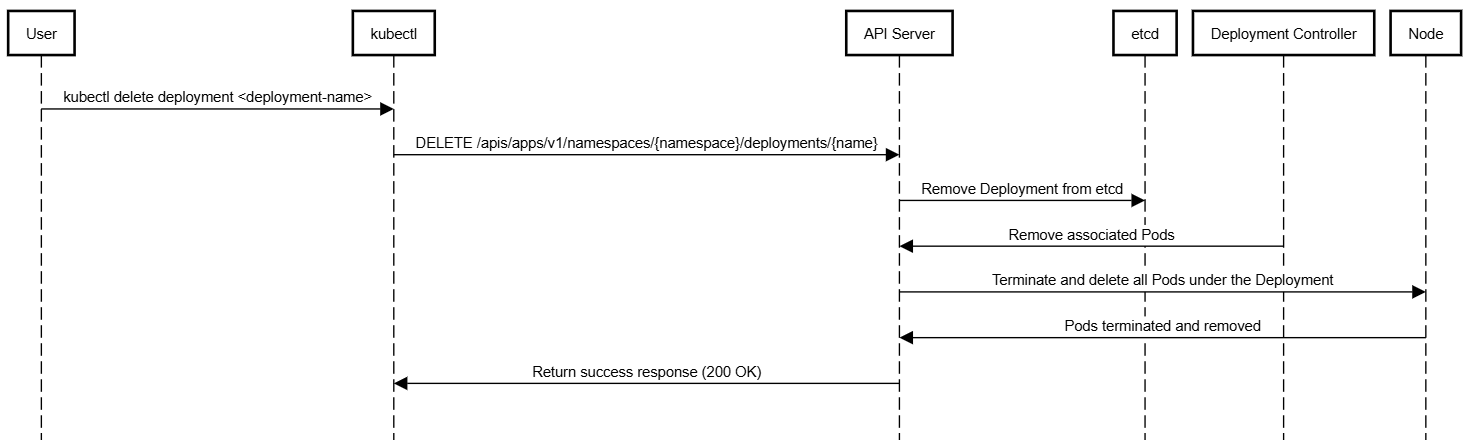
\includegraphics[width=\textwidth]{uml_diagrams/create_deployment.png}
    \caption{Creating a Deployment}
    \label{fig:create_deployment_diagram}
\end{figure}

During validation, if the YAML file has missing or invalid fields (e.g., no container image specified), or if the user lacks the necessary permissions, the API detects this error, and returns one the following error codes: 
\begin{itemize}
    \item 400 Bad Request: If the YAML syntax or required fields are incorrect.
    \item 403 Forbidden: If the user lacks permissions to create resources in the specified namespace.
    \item 409 Conflict: If a Pod with the same name already exists in the namespace.
\end{itemize}

\begin{figure}[H]
    \centering
    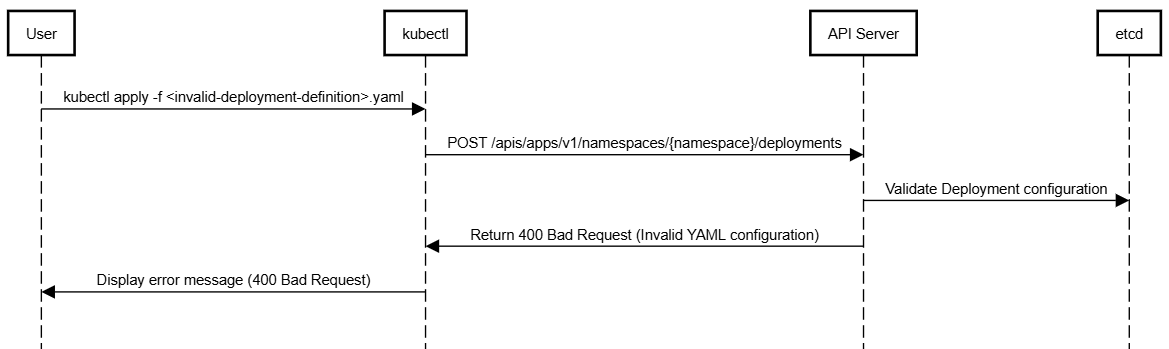
\includegraphics[width=\textwidth]{uml_diagrams/error_creating.png}
    \caption{Error During Creating a Deployment}
    \label{fig:create_deployment_diagram}
\end{figure}



\subsection{Checking Pod Status}
The user can check the status of a specific Pod by the following command: \texttt{kubectl get pod <pod-name>}, which translates to  \texttt{GET /api/v1/namespaces/{namespace}/pods/{name}}. The API server queries etcd for the latest data on the specified Pod, including its current state (Pending, Running, Succeeded, Failed, or Unknown), then it sends back a structured JSON response.
The Pod must exist in the specified namespace, otherwise a 404 Not Found error is sent back.
\begin{figure}[H]
    \centering
    \includegraphics[width=\textwidth]{uml_diagrams/check_pod.png}
    \caption{Checking Pod Status}
    \label{fig:create_deployment_diagram}
\end{figure}

\subsection{Delete or Restart a Pod}
In Kubernetes, deleting a Pod managed by a controller, such as a Deployment or ReplicaSet, usually results in restarting the Pod. This is because controllers automatically recreate deleted Pods to maintain the desired replica count. If the intent is to restart the Pod, deleting it will suffice. However, to permanently delete it without triggering a recreation, user must either scale the replicas down to zero or delete the Deployment itself.

\subsubsection{Restart a Pod}
The user can restart a Pod by issuing  \texttt{kubectl delete pod <pod-name>}, which translates to \texttt{DELETE \newline /api/v1/namespaces/{namespace}/pods/{name}}. The API server processes the request and initiates the Pod’s deletion, marking it as Terminating.
The Deployment or ReplicaSet controller detects that a Pod is missing and creates a new Pod to maintain the desired replica count.
The new Pod enters the Pending state, then moves to Running once the containers start successfully.
The Pod must exist and be accessible within the specified namespace, otherwise otherwise a 404 Not Found error is sent back.
\begin{figure}[H]
    \centering
    \includegraphics[width=\textwidth]{uml_diagrams/restart_pod.png}
    \caption{Restarting a Pod}
    \label{fig:create_deployment_diagram}
\end{figure}

\subsubsection{Delete a Pod}
To permanently delete a managed Pod, the first way is to issue \texttt{kubectl scale deployment <deployment-name> --replicas=0}, which sends a PATCH request to the API Server to update the replica count. 
\begin{figure}[H]
    \centering
    \includegraphics[width=\textwidth]{uml_diagrams/scale_down.png}
    \caption{Scale Down a Deployment}
    \label{fig:create_deployment_diagram}
\end{figure}


The other way is to delete the deployment wit \texttt{kubectl delete deployment <deployment-name>}, which sends a DELETE request to the API Server to remove the Deployment. The API server processes the request, updating the Deployment state in etcd.
The controller deletes any remaining Pods associated with the Deployment and does not recreate them.
\begin{figure}[H]
    \centering
    \includegraphics[width=\textwidth]{uml_diagrams/delete_deployment.png}
    \caption{Deleting Deployment}
    \label{fig:create_deployment_diagram}
\end{figure}

\paragraph{Note:}
It is also possible to force delete a pod, if a  \texttt{--grace-period=0 --force} flag is provided to the \texttt{kubectl} command. It allows the user to immediately terminate a Pod without waiting for a graceful shutdown period.



\end{document}